%% Do not edit preable unless you know what you are doing.
\documentclass{article}\usepackage[]{graphicx}\usepackage[]{color}
% maxwidth is the original width if it is less than linewidth
% otherwise use linewidth (to make sure the graphics do not exceed the margin)
\makeatletter
\def\maxwidth{ %
  \ifdim\Gin@nat@width>\linewidth
    \linewidth
  \else
    \Gin@nat@width
  \fi
}
\makeatother

\definecolor{fgcolor}{rgb}{0.345, 0.345, 0.345}
\newcommand{\hlnum}[1]{\textcolor[rgb]{0.686,0.059,0.569}{#1}}%
\newcommand{\hlstr}[1]{\textcolor[rgb]{0.192,0.494,0.8}{#1}}%
\newcommand{\hlcom}[1]{\textcolor[rgb]{0.678,0.584,0.686}{\textit{#1}}}%
\newcommand{\hlopt}[1]{\textcolor[rgb]{0,0,0}{#1}}%
\newcommand{\hlstd}[1]{\textcolor[rgb]{0.345,0.345,0.345}{#1}}%
\newcommand{\hlkwa}[1]{\textcolor[rgb]{0.161,0.373,0.58}{\textbf{#1}}}%
\newcommand{\hlkwb}[1]{\textcolor[rgb]{0.69,0.353,0.396}{#1}}%
\newcommand{\hlkwc}[1]{\textcolor[rgb]{0.333,0.667,0.333}{#1}}%
\newcommand{\hlkwd}[1]{\textcolor[rgb]{0.737,0.353,0.396}{\textbf{#1}}}%
\let\hlipl\hlkwb

\usepackage{framed}
\makeatletter
\newenvironment{kframe}{%
 \def\at@end@of@kframe{}%
 \ifinner\ifhmode%
  \def\at@end@of@kframe{\end{minipage}}%
  \begin{minipage}{\columnwidth}%
 \fi\fi%
 \def\FrameCommand##1{\hskip\@totalleftmargin \hskip-\fboxsep
 \colorbox{shadecolor}{##1}\hskip-\fboxsep
     % There is no \\@totalrightmargin, so:
     \hskip-\linewidth \hskip-\@totalleftmargin \hskip\columnwidth}%
 \MakeFramed {\advance\hsize-\width
   \@totalleftmargin\z@ \linewidth\hsize
   \@setminipage}}%
 {\par\unskip\endMakeFramed%
 \at@end@of@kframe}
\makeatother

\definecolor{shadecolor}{rgb}{.97, .97, .97}
\definecolor{messagecolor}{rgb}{0, 0, 0}
\definecolor{warningcolor}{rgb}{1, 0, 1}
\definecolor{errorcolor}{rgb}{1, 0, 0}
\newenvironment{knitrout}{}{} % an empty environment to be redefined in TeX

\usepackage{alltt}
\usepackage[sc]{mathpazo}
\usepackage[T1]{fontenc}
\usepackage[english]{babel}
\usepackage[utf8]{inputenc}
\usepackage{geometry}
\usepackage{dsfont}
\usepackage{indentfirst}
\usepackage{fancyhdr}
\usepackage{amsmath}
\usepackage{enumitem}

% No indents in whole document
\setlength\parindent{0pt}

% Gaps between item is itemize
\setitemize{itemsep=-1em,topsep=0.5em,parsep=0em,partopsep=0pt}

% Margins of the document
\geometry{verbose,tmargin=2.5cm,bmargin=2.5cm,lmargin=2.5cm,rmargin=2.5cm}

% Header and footer for all pages
\pagestyle{fancy}
\fancyhf{}
\renewcommand{\headrulewidth}{0pt}
\rfoot{Page \thepage}

% Header and footer for first page
\fancypagestyle{plain}{%
  \renewcommand{\headrulewidth}{0pt}%
  \fancyhf{}%
  \rhead{ETH Zurich}
  \lhead{Applied Generalized Linear Models \\ Spring Semester 2020}
  \rfoot{Page \thepage}
}

% Global Settings of R-code


% Mathematics Operators for Ease of Notation
\DeclareMathOperator{\SSR}{SSR}
\DeclareMathOperator{\SSreg}{SSreg}
\DeclareMathOperator{\SST}{SST}

% Bad Box settings
\hbadness=10000
\vbadness=\maxdimen
\vfuzz=30pt
\hfuzz=30pt


%% ---------- BEGIN DOCUMENT -----------------------------------------------
\IfFileExists{upquote.sty}{\usepackage{upquote}}{}
\begin{document}

%% Tiltle
\title{Assignment 1}
\author{Milan Kuzmanovic, Mark McMahon \\ Martin Kotuliak, Jakub Polak}
\date{\today}
\maketitle

\section*{Task 1}

A multiple linear regression model has been estimated to study the relation- ship between $Y =$ violent crime rate (per 100,000 people), $X_1 =$ poverty rate (percentage with income below the poverty line) and $X_2 =$ percentage living in urban area. Data are collected in 51 cities in the U.S.\\

The relevant equations that relate estimate, standard error, T-statistic, R-squared and Sum of Squares of residuals, regression and total are folloqwing.

\[ \frac{\beta_i}{se(\beta_i)} = T_i \qquad R^2 = \frac{\SSreg}{\SST}= 1-\frac{\SSR}{\SST}  \qquad \SST = \SSreg + \SSR
\]

Using these we just plug in the corresponding information that is already provided and compute the missing values.

\begin{knitrout}
\definecolor{shadecolor}{rgb}{0.969, 0.969, 0.969}\color{fgcolor}\begin{kframe}
\begin{alltt}
\hlstd{a} \hlkwb{<-} \hlopt{-}\hlnum{498.683} \hlopt{/} \hlnum{140.988}
\hlstd{b} \hlkwb{<-} \hlnum{4.885} \hlopt{*} \hlnum{6.677}
\hlstd{c} \hlkwb{<-} \hlnum{9.112} \hlopt{/} \hlnum{6.900}
\hlstd{d} \hlkwb{<-} \hlnum{1841257.15} \hlopt{/} \hlstd{(}\hlnum{1} \hlopt{-} \hlnum{0.5708}\hlstd{)}
\hlstd{e} \hlkwb{<-} \hlstd{d} \hlopt{-} \hlnum{1841257.15}
\end{alltt}
\end{kframe}
\end{knitrout}

The table below reports the output with filled in missing information.

\begin{center}
\begin{tabular}{ l r r r r }
 \hline
            & Est.            & s.e.              & t-value         & p-value \\
 \hline
 Intercept  & -498.683  & 140.988 & $^{a\;}$-3.537 & 0.009 \\
 $X_1$      & $^{b\;}$32.617 & 6.677  & 4.885     & 0.001 \\
 $X_2$      & 9.112  & $^{c\;}$1.321 & 6.900      & 0.001 \\
 \hline
 $R^2$      & 0.5708            & & & \\
 SSreg      & $^{e\;}$2448718 & & & \\
 SSR        & 1841257.15        & & & \\
 SSTotal    & $^{d\;}$4289975 & & & \\
 \hline
\end{tabular}
\end{center}

The the coefficient of determination $R^2$ is $0.5708$. This value measures the proportion of the variance in $Y$ explained by the model. Hence, 57.08 \% of the sample variability of $Y$ can be explained by the linear combination of $X_i$'S given the sample data.\\

To compute the overall F-test we use the equation below and the statistic then follows an F distribution with corresponding degrees of freedom.
\[ F = \frac{\SSreg/p}{\SSR/(n-(p+1))} \sim F_{p,n-(p+1)}
\]

The data are collected in 51 cities, so $n=51$ and we have 2 predictors, so $p=2$. Other values we can easily obtain from the filled table above.
\begin{knitrout}
\definecolor{shadecolor}{rgb}{0.969, 0.969, 0.969}\color{fgcolor}\begin{kframe}
\begin{alltt}
\hlstd{(f} \hlkwb{=} \hlstd{(e} \hlopt{/} \hlnum{2}\hlstd{)} \hlopt{/} \hlstd{(}\hlnum{181257.15} \hlopt{/} \hlstd{(}\hlnum{51}\hlopt{-}\hlstd{(}\hlnum{2}\hlopt{+}\hlnum{1}\hlstd{)) ))}
\end{alltt}
\begin{verbatim}
## [1] 324.2312
\end{verbatim}
\end{kframe}
\end{knitrout}

Hence, the F-statistic has a value of 324.2311914. To interpret this, the global F-test, tests a null hypothesis that all regression coefficients are simultaneously 0. In a mathematical notation $H_0 : \beta_1 = \beta_2 = 0$. To evaluate the test, we can compute its p-value. It is a quantile of the corresponding F-distribution for the given statistic or mass under the distribution.

\begin{knitrout}
\definecolor{shadecolor}{rgb}{0.969, 0.969, 0.969}\color{fgcolor}\begin{kframe}
\begin{alltt}
\hlstd{(p} \hlkwb{=} \hlkwd{pf}\hlstd{(f,}\hlnum{2}\hlstd{,}\hlnum{48}\hlstd{,}\hlkwc{lower.tail} \hlstd{=} \hlnum{FALSE}\hlstd{))}
\end{alltt}
\begin{verbatim}
## [1] 1.319003e-28
\end{verbatim}
\end{kframe}
\end{knitrout}

The p-value is \ensuremath{1.3190029\times 10^{-28}}, which is very low and therefore there is a significant evidence against the null hypothesis that all regression coefficients are simultaneously zero. Hence, the p-value of a given sample is small and it suggests that the model with all the covariates is better than the one with just intercept coefficient. This test therefore determines if the linear model is at least suitable to explain some of the variance in the outcome variable. Which in this case it does.

\section*{Task 2}

The table below shows the scores of the first test (maximum score 10 points) in a beginning German course. Students in the course are grouped as follows:
\begin{itemize}
\item Group A: Never studied foreign language before, but have good English skills\\
\item Group B: Never studied foreign language before, have poor English skills\\
\item Group C: Studied other foreign language
\end{itemize}

\begin{center}
\begin{tabular}{ c c c }
 \hline
 Group A & Group B & Group C \\
 \hline
 4 & 1 & 9 \\
 6 & 5 & 10 \\
 8 &   & 5 \\
 \hline
\end{tabular}
\end{center}

Two-sample t-test is usual method for comparing mean scores of two groups. The one-way analysis of variance (ANOVA), also known as one-factor ANOVA, is an extension of independent two-samples t-test for comparing means in a situation where there are more than two groups. This corresponds to our situation.\\

The Hypothesis test in ANOVA is following:
\begin{itemize}
\item Null hypothesis: the means of the different groups are the same \\
\item Alternative hypothesis: At least one sample mean is not equal to the others
\end{itemize}

The Assumptions of ANOVA are following:
\begin{itemize}
\item The observations are obtained independently and randomly from the population defined by the groups of factor levels.\\
\item The data of each factor level are normally distributed.\\
\item These normal populations have a common variance.
\end{itemize}

The F-test is used for comparing the factors of the total deviation. In ANOVA, F-statistic is computed as the ratio of the variance between groups and variance within groups. The F-statistic is then compared to the F-distribution with $I-1$ and $n-I$ degrees of freedom, where $I =$ total number of groups and $n =$ total number of observations. Note that, a lower ratio (ratio $< 1$) indicates that there are no significant difference between the means of the samples being compared. However, a higher ratio implies that the variation among group means are significant.\\

The process of ANOVA testing is following:
\begin{itemize}
\item Compute the common variance, which is called variance within samples $S^2_{\text{within}}$ or residual variance.\\
\item Compute the variance between sample means, by first computing the mean of each group and then computing the variance between sample means . \\
\item Produce F-statistic as the ratio of $F =S^2_{\text{between}} / S^2_{\text{within}}$.
\end{itemize}

With the code below, we specify the data and compute common statistics for each group.
\begin{knitrout}
\definecolor{shadecolor}{rgb}{0.969, 0.969, 0.969}\color{fgcolor}\begin{kframe}
\begin{alltt}
\hlstd{X} \hlkwb{<-} \hlkwd{data.frame}\hlstd{(}\hlstr{"grade"} \hlstd{=} \hlkwd{c}\hlstd{(}\hlnum{4}\hlstd{,}\hlnum{6}\hlstd{,}\hlnum{8}\hlstd{,}\hlnum{1}\hlstd{,}\hlnum{5}\hlstd{,}\hlnum{9}\hlstd{,}\hlnum{10}\hlstd{,}\hlnum{5}\hlstd{),}
                \hlstr{"group"} \hlstd{=} \hlkwd{c}\hlstd{(}\hlstr{"A"}\hlstd{,}\hlstr{"A"}\hlstd{,}\hlstr{"A"}\hlstd{,}\hlstr{"B"}\hlstd{,}\hlstr{"B"}\hlstd{,}\hlstr{"C"}\hlstd{,}\hlstr{"C"}\hlstd{,}\hlstr{"C"}\hlstd{))}
\hlkwd{library}\hlstd{(dplyr)}
\hlkwd{data.frame}\hlstd{(}\hlkwd{group_by}\hlstd{(X, group)} \hlopt
  \hlkwd{summarise}\hlstd{(} \hlkwc{count} \hlstd{=} \hlkwd{n}\hlstd{(),} \hlkwc{mean} \hlstd{=} \hlkwd{mean}\hlstd{(grade),} \hlkwc{var} \hlstd{=} \hlkwd{var}\hlstd{(grade),} \hlkwc{sd} \hlstd{=} \hlkwd{sd}\hlstd{(grade)))}
\end{alltt}
\begin{verbatim}
##   group count mean var       sd
## 1     A     3    6   4 2.000000
## 2     B     2    3   8 2.828427
## 3     C     3    8   7 2.645751
\end{verbatim}
\end{kframe}
\end{knitrout}

These can be easily visualised with a boxplot (left) or a group means plot with errorbars signifying one standard deviation (right). The main observation we conclude from these plot is the large variance within groups caused mainly by having just few observations.

\begin{knitrout}
\definecolor{shadecolor}{rgb}{0.969, 0.969, 0.969}\color{fgcolor}

{\centering 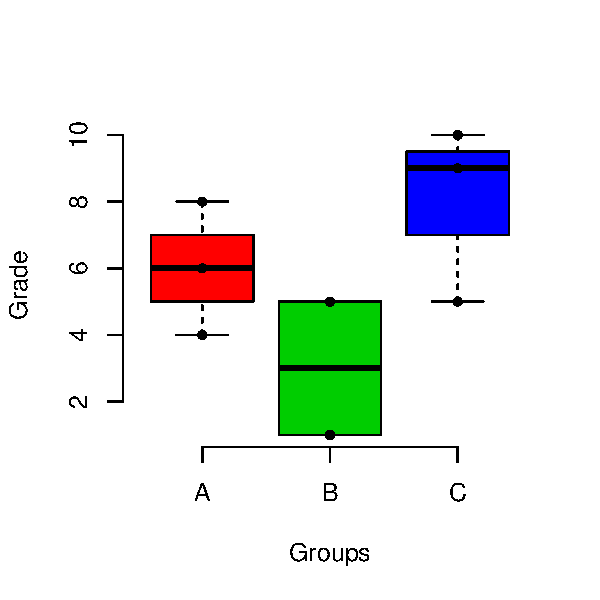
\includegraphics[width=.4\linewidth]{figures/plot-t2-plots-1} 
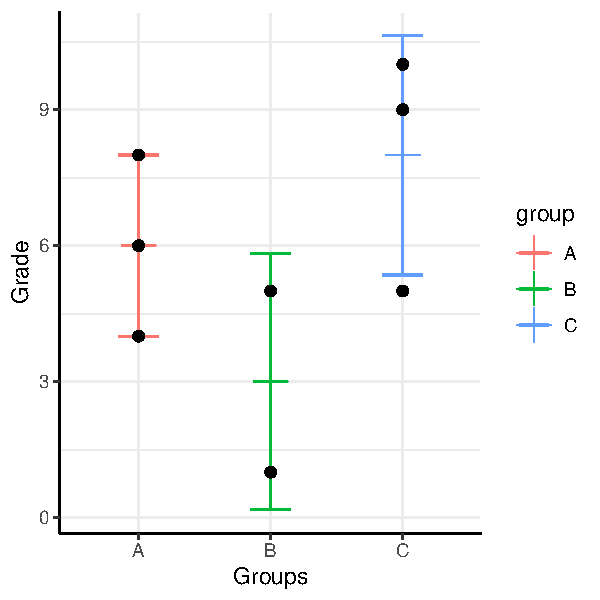
\includegraphics[width=.4\linewidth]{figures/plot-t2-plots-2} 

}



\end{knitrout}

Finaly, below we compute the ANOVA tests with our data using the function \verb+aov()+.

\begin{knitrout}
\definecolor{shadecolor}{rgb}{0.969, 0.969, 0.969}\color{fgcolor}\begin{kframe}
\begin{alltt}
\hlstd{fit} \hlkwb{<-} \hlkwd{aov}\hlstd{(grade} \hlopt{~} \hlstd{group,} \hlkwc{data} \hlstd{= X)}
\hlkwd{summary}\hlstd{(fit)}
\end{alltt}
\begin{verbatim}
##             Df Sum Sq Mean Sq F value Pr(>F)
## group        2     30      15     2.5  0.177
## Residuals    5     30       6
\end{verbatim}
\end{kframe}
\end{knitrout}

The F-statistics has value of 2.5, which is above 1 which signifies some differences in group means. However the p-value is 0.177, which is not signigicant under the 5 \% significance level and therefore we cannot reject the null hypothesis of the group means being different.

\begin{knitrout}
\definecolor{shadecolor}{rgb}{0.969, 0.969, 0.969}\color{fgcolor}\begin{kframe}
\begin{verbatim}
##             Df Sum Sq Mean Sq F value Pr(>F)
## group        2      6       3     0.5  0.634
## Residuals    5     30       6
##             Df Sum Sq Mean Sq F value Pr(>F)  
## group        2  30.00  15.000   7.249 0.0333 *
## Residuals    5  10.35   2.069                 
## ---
## Signif. codes:  0 '***' 0.001 '**' 0.01 '*' 0.05 '.' 0.1 ' ' 1
##             Df Sum Sq Mean Sq F value  Pr(>F)    
## group        2  298.0  149.02   24.22 6.9e-09 ***
## Residuals   77  473.7    6.15                    
## ---
## Signif. codes:  0 '***' 0.001 '**' 0.01 '*' 0.05 '.' 0.1 ' ' 1
\end{verbatim}
\end{kframe}
\end{knitrout}

Case:Suppose that the first observation in the second group was actually 9, not 1. Then, the standard deviations are the same, but the sample means are 6, 7 and 8, rather than 6, 3 and 8.\\

In this situation, we would expect the


\section*{Task 3}

\section*{Task 4}

\section*{Task Template}

This is just an expample of how to use latex and r-code chunks in knitr.\\

You can test if \textbf{knitr} works with this minimal demo. OK, let's
get started with some boring random numbers:

\begin{knitrout}
\definecolor{shadecolor}{rgb}{0.969, 0.969, 0.969}\color{fgcolor}\begin{kframe}
\begin{alltt}
\hlkwd{set.seed}\hlstd{(}\hlnum{1121}\hlstd{)}
\hlstd{(x}\hlkwb{=}\hlkwd{rnorm}\hlstd{(}\hlnum{20}\hlstd{))}
\end{alltt}
\begin{verbatim}
##  [1]  0.1449583  0.4383221  0.1531912  1.0849426  1.9995449 -0.8118832  0.1602680
##  [8]  0.5858923  0.3600880 -0.0253084  0.1508809  0.1100824  1.3596812 -0.3269946
## [15] -0.7163819  1.8097690  0.5084011 -0.5274603  0.1327188 -0.1559430
\end{verbatim}
\begin{alltt}
\hlkwd{mean}\hlstd{(x);}\hlkwd{var}\hlstd{(x)}
\end{alltt}
\begin{verbatim}
## [1] 0.3217385
## [1] 0.5714534
\end{verbatim}
\end{kframe}
\end{knitrout}

The first element of \texttt{x} is 0.1449583. Boring boxplots
and histograms recorded by the PDF device:

\begin{knitrout}
\definecolor{shadecolor}{rgb}{0.969, 0.969, 0.969}\color{fgcolor}\begin{kframe}
\begin{alltt}
\hlkwd{par}\hlstd{(}\hlkwc{mar}\hlstd{=}\hlkwd{c}\hlstd{(}\hlnum{4}\hlstd{,}\hlnum{4}\hlstd{,}\hlnum{.1}\hlstd{,}\hlnum{.1}\hlstd{),}\hlkwc{cex.lab}\hlstd{=}\hlnum{.95}\hlstd{,}\hlkwc{cex.axis}\hlstd{=}\hlnum{.9}\hlstd{,}\hlkwc{mgp}\hlstd{=}\hlkwd{c}\hlstd{(}\hlnum{2}\hlstd{,}\hlnum{.7}\hlstd{,}\hlnum{0}\hlstd{),}\hlkwc{tcl}\hlstd{=}\hlopt{-}\hlnum{.3}\hlstd{,}\hlkwc{las}\hlstd{=}\hlnum{1}\hlstd{)}
\hlkwd{boxplot}\hlstd{(x)}
\hlkwd{hist}\hlstd{(x,}\hlkwc{main}\hlstd{=}\hlstr{''}\hlstd{)}
\end{alltt}
\end{kframe}

{\centering 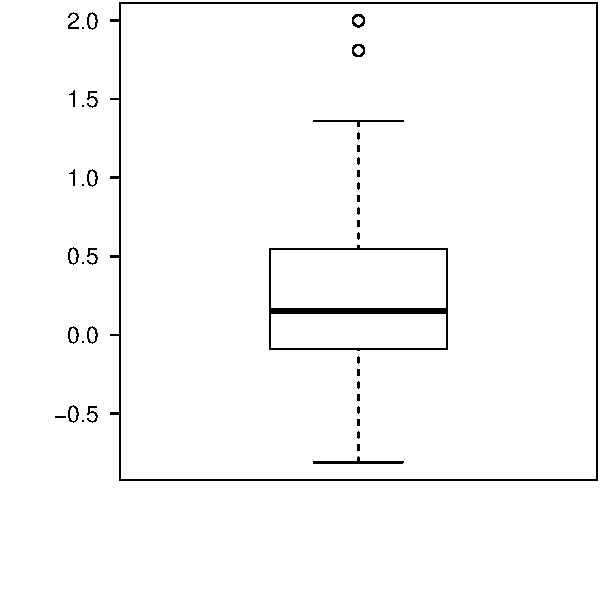
\includegraphics[width=.4\linewidth]{figures/plot-boring-plots-1} 
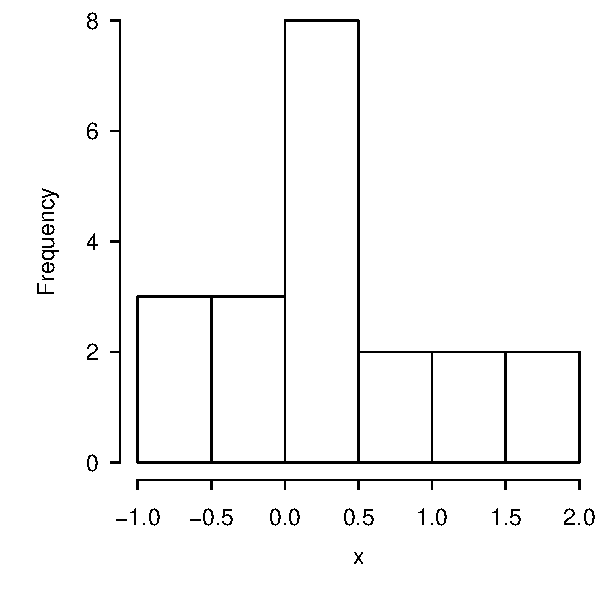
\includegraphics[width=.4\linewidth]{figures/plot-boring-plots-2} 

}



\end{knitrout}

Do the above chunks work? You should be able to compile the \TeX{}
The first element of \texttt{x} is 0.1449583. Boring boxplots
and histograms recorded by the PDF device:

\begin{knitrout}
\definecolor{shadecolor}{rgb}{0.969, 0.969, 0.969}\color{fgcolor}

{\centering 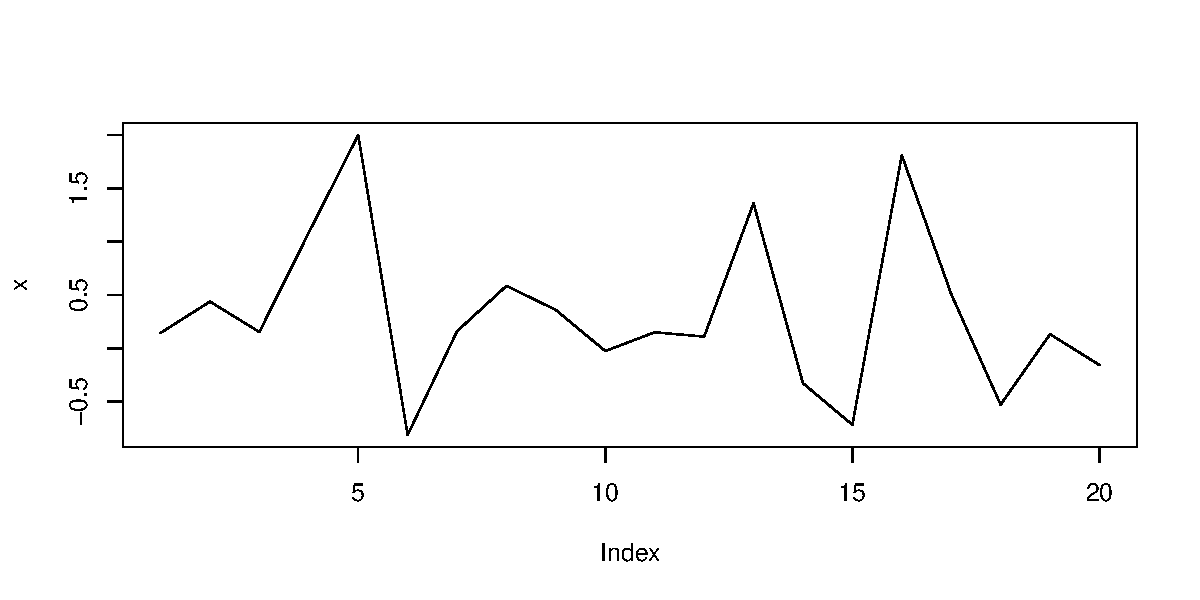
\includegraphics[width=.8\linewidth]{figures/plot-boring-plots2-1} 

}



\end{knitrout}

Do the above chunks work? You should be able to compile the \TeX{}

\end{document}
